
\documentclass{aa}  

\usepackage{graphicx}
%%%%%%%%%%%%%%%%%%%%%%%%%%%%%%%%%%%%%%%%
\usepackage{txfonts}
%%%%%%%%%%%%%%%%%%%%%%%%%%%%%%%%%%%%%%%%
%\usepackage[options]{hyperref}
% To add links in your PDF file, use the package "hyperref"
% with options according to your LaTeX or PDFLaTeX drivers.
%
\begin{document} 


   \title{The data center for the X-ray Imaging Spectrometer/Telescope STIX}

   \subtitle{}

   \author{H. Xiao
          \inst{1}
          \and 
          Shane Maloney 
          \inst{2}
          \and 
          Ewan Dickson \inst{1,4}
          \and 
          S\"am Krucker\inst{1}
            \and László Etesi \inst{1}
          \and Andrea Francesco Battaglia\inst{1,3}
          \and Daniel Ryan\inst{1}
          \and Other STIX team members
         }

   \institute{University of Applied Sciences and Arts Northwestern Switzerland (FHNW), 5200 Windisch, Switzerland \\
              \email{hualin.xiao@fhnw.ch}
         \and
          Astrophysics Research Group, School of Physics, Trinity College Dublin, Dublin 2, Ireland
          \and
             ETH Z\"urich, R\"amistrasse 101, 8092 Z\"urich, Switzerland
         \and University of Graz, Universitätspl. 3, 8010 Graz, Austria
             }

   \date{}

% \abstract{}{}{}{}{} 
% 5 {} token are mandatory
 
  \abstract
  % context heading (optional)
   {} %leave it empty if necessary  
  % {context.}
  % aims heading (mandatory)
   { The Spectrometer/Telescope for Imaging X-rays (STIX) instrument onboard the Solar Orbiter mission launched on February 10, 2020 promises advances in the study of solar flares of various sizes. It is capable of measuring X-ray spectra from 4 to 150 keV with 1 keV resolution binned into 32 energy bins before downlinking. STIX data center is an infrastructure established at FHNW in order to process and archive STIX telemetry data, and to support the operations of the instrument. The automated data processing pipeline turns raw telemetry data into processed information and data products. Processed information and data products are achived at the data center.  STIX data center provides various tools to visualized the information and data products for the solar physics community.
   }
  % methods heading (mandatory)
   {Methods}
  % results heading (mandatory)
   {Results.}
  % conclusions heading (optional), leave it empty if necessary 
   {}

   \keywords{Solar flares --Data Center --
                STIX data products --
                Data processing pipeline
               }

   \maketitle
%
%-------------------------------------------------------------------

\section{Introduction}
Solar Orbiter is a Sun-observing mission of the European Space  Agency that 
addresses the interaction between the Sun and the heliosphere.
It was lunched on Feb. 10, 2020 for a nominal mission duration of seven years and a planned 
extension of
three years. It carries ten sets of instruments for comprehensive
remote-sensing and in-situ measurements. 
Solar Orbiter  will perform detailed measurements of the Sun as close as 0.28 AU and for the first time look at its uncharted polar regions (\cite{SolarOrbiter2020}).  
Its goal is to  address the center question of heliophysics  "How does the Sun create and control the heliosphere?".  It is designed to identify the origins and causes of the solar wind, the heliospheric magnetic field, the solar energetic particles, the transient interplanetary disturbances, and the Sun's magnetic field.
This consists of the study of energetic solar phenomena like flares,  solar transients,  the solar wind accelerating mechanisms, and the solar dynamo principle.  


The Spectrometer Telescope for Imaging X-rays (STIX) is one of the ten instruments onboard Solar Orbiter.  It measures X-rays from 4 to 150 keV and takes X-ray images with a few arcsec angular resolution by using an indirect imaging technique, based on the Moiré effect .  The angular resolution
is 7 arcsec and the spectral resolution 1.1 keV full-width-half-maximum at 30 keV.
Its instrument consists of 32 collimators with
grids and 32 pixelated Cadmium telluride  detector units called Caliste-SO  \cite{StixInstrument}.
STIX's main purpose is to study the extremely hot solar plasma and the high-energy electrons accelerated during solar flares.
It will address the key science goals of the Solar Orbiter mission by providing information on intensity, spectrum, timing, and location of accelerated electrons near the Sun. 


STIX has more than two hundred different telemetry data types. The data
have complex data structures and are higly compressed.
Being aware of the complexity of the data analysis and of
the need to bring the data to the community, a data center is
developed at FHNW in order to receive, analyze,  archive and distribute the STIX data.
The data center turns raw telemetry data into processed information and data products that can be used for scientific analysis.
SDC also provides various data visualization the solar physics comunity.
We will describe here STIX raw data types, the flow of data from to the users, the main data processing steps, the data products and the tools provided for the comnunity.


%--------------------------------------------------------------------
\section{STIX raw telemetry data}

\begin{figure}
    \centering
    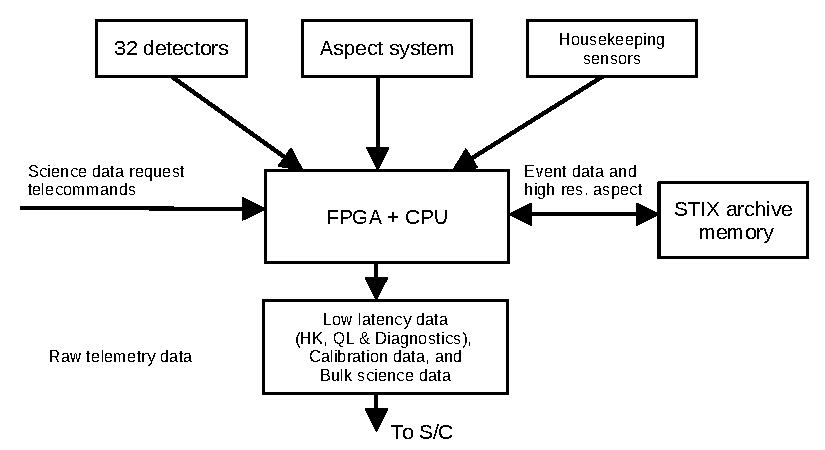
\includegraphics[width=0.8\linewidth]{figures/onboardDataFlow.pdf}
    \caption{STIX onboard data flow and data types.}
    \label{fig:stix_onbard_data_flow}
\end{figure}

During the nomal operation, STIX continously collects data from the 32 x-ray detector units, the aspect system and
housekeeping sensors.
The event data from the x-ray detetors are processed in three parallel paths:
1) a primary data path transfer time-binned event data to the instrument archive memory;
2) a quick-look path generates light curves, snapshots of energy spectra and flare triggers;
3) a calibration path collects events during quiet periods and uses them to form calibration spectrum for each pixel;


Event data and high time resolution aspect
readouts are stored in STIX archive flash memory.
The processed data is  stored on the on-board archive memory for further processing as requested by ground commanding, or used to form telemetry data packets.
As shown in  STIX raw telemetry data can be classified in four categories: Housekeeping (HK), Quick-look (QL), Diagnostic
, and user requested bulk science data.
HK data and QL data are directed to the low latency data store in
the Solid State Mass Memory (SSMM) of the spacecraft. They are sent down to Earth when during ground antenna passes.



\section{Overview of the data flow}
STIX telemetry data are first be stored in the spacecraft solid state disk.
They are transmitted to ground stations during antenna passes.
Telemetry data recieved by ground stations are processed at the mission control center of ESA and
stored in .
ESA provides a web interface.
The typical latency of the low latency data before they arrive at STIX data center is about x day when there is a pass a.
Raw data received at STIX data center has the same structure.

The payload data must be created through the EEDS web page to create a data download request. After receiving the user's data request, EDDS displays the original payload data in the form of hex code and sends it to the stix data center server through the RSYNC protocol. Users can define the time interval of data request. Generally speaking, STIX server requests data from EDDS once a day. The data STIX obtains from EDDS is a HEX code with a time stamp, which is the same as the data sent by STIX to the spacecraft platform after being converted into binary data.

In addition to telemetry data, STIX data center also receive spacecraft ancillary data from ESA, that contains
information of spacecraft ephemris and factors for time conversion.


\section{Data processing pipelines at STIX data center}



\subsection{Data link and data reception}

\subsection{STIX raw data processing pipeline}
\subsubsection{Raw data parsing}

include a decompression error map here
\subsubsection{Background monitoring}
Light curves measured during quiet periods of the sun are used for background estimation. Median values and of counts are computed and considered as the background in the selected time frame. They are stored in a database and used for flare identifications. 
\subsubsection{Flare identification}
Quick-look light curves in the energy range 4 to 10 keV are used for solar flare identification.  The flare identification procedure consists of  two steps:
\begin{itemize}
\item Light curve smoothing. In order to filter spikes from electronics and to reduce the amount of variation due to statistics and the onboard integer compression, light curves are smoothed by using the average filtering. The 
\item Flare identification. Local maximums are selected from smoothed light curves.  A local maximum is considered as a flare peak if the counts are exceeds 2 standard deviations above the background and the duration above the background is longer than 1 minute.  
\end{itemize}

For each of identified solar flares,   the  information such as start time, end time, counts, background subtracted counts is stored in the STIX flare database.   It is used for automatic creation of data requests for on-board archived data. 

\subsubsection{flare ID naming convention}
\subsubsection{Flare locations}
\subsection{Calibration data processing}

Ba134 radioactive sources with a total activity of about 4000 Bq are placed at the front of each detector. The total activity of the radioactive source is approximately 4000 Ba.
When the radioactive source decays, gamma rays are generated. These gamma rays can form peaks in the energy spectrum of the detector.
The corresponding energy is known, and the corresponding relationship between ADC and real energy can be calibrated through the position of the peak in the energy spectrum, that is, the calibration coefficient. The figure below is a typical Ba133 gamma-ray energy spectrum measured by STIX CdTe detector. There are three obvious peaks in the energy spectrum, and they correspond to three energies of 30 keV, 35 keV and 81 keV. There are many ways to determine the position of each peak, you can use the ECC method, or use the Gaussian function to fit the left part of the peak.

\subsubsection{Flare location using coarse flare data}
\subsubsection{Flare classification using GOES x-ray flux}
\subsubsection{FITS file creation}
\section{STIX data products}
\begin{itemize}
    \item Raw data.
    \item L1 data.
    \item L2 data
    
\end{itemize}

The latest level 1 FITS IO from Shane has been integrated into the data processing pipeline on pub023 server.

I have recreated fits products for all old telemetry data with the upgraded SW.

The L1 fits files  created by this pipeline have a different data level:  L1A ('A' here means  prerelease/alpha version).

The idea behind L1A data sets is to allow for quicker access to STIX data in the fits format instead of grabbing  data from plots or using JSON requests,

for operations,  debugging  etc.

The L1A data sets can be generated within a few minutes after the arrival of a new raw telemetry file.

The differences between L1A and L1 available in Shane's ftp include:

1.  Two different L1A data files may have duplicated data

2.  L1A data sets are still created for incomplete packets  (L1 checks for data completeness)

3.  SPICE kernel data for telemetry files always arrives  after one or two days later.
    So  there may be a sub-second difference between the UTC time in fits files (same to times on web pages)

   and the real time.

    Shane's formal L1 release can avoid this issue if they are produced on a later date.

4. L1A contains housekeeping data




The Level0 archive contains TM which has been parsed or decommuated into readable structures but no additional external information is include:

times are not converted to UTC
no calibration or conversions applied
for STIX we need to decide if we decompress / combine X-ray L0 the count/trigger data at this stage or in the next level L1

copy manual,
tree like, 
json formats
name, raw value, eng value, children
look-up table, to know description

estimate mongodb benchmark
Mongodb benchmark,
key value, index, performance



\begin{table}
\centering
\caption{Level 1 data products}
\begin{tabular}{llll}
Category & Type   &  Naming convention  & Remarks   \\ \hline
 Housekeeping & hk\_mini  &  & Houskeeping in BOOT mode   \\
 & hk\_maxi  &  & houskeeping data in NOMINAL   \\
 Quick-look &  light curves &  & Quicklook lightcurves \\
  &  variance &  & variance \\
  &  spectra &  &  \\
  &  background monitor &  &  \\
    &  flare location &  &  \\
 Calibration data &   &  &  \\
\end{tabular}
\end{table}

\section{Data request procedure}
created of data requests
manuall checked
\textbf{  data request naming convention  yyddmm00  to yyddmm 11 }


\section{Flare processing}

\section{Database}
\subsection{Raw data packet database } 
\subsection{Configuration database}

\section{Online data visualization tools}
\subsection{Quick-look light curve}
\subsection{Science data quick analysis}
\subsubsection{Calibration data}
\begin{figure}
    \centering
    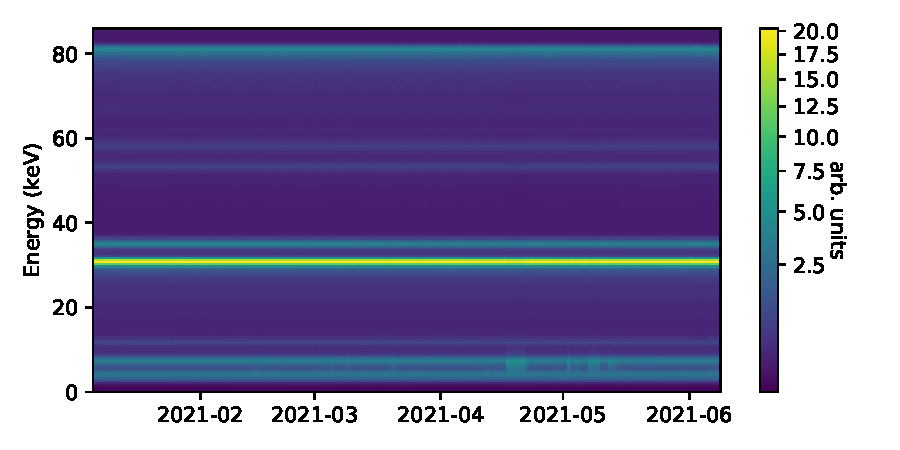
\includegraphics[width=0.8\linewidth]{figures/calibrationSpectrogram.pdf}
    \caption{Caption}
    \label{fig:calibrationSpectrum}
\end{figure}
\begin{figure}
    \centering
    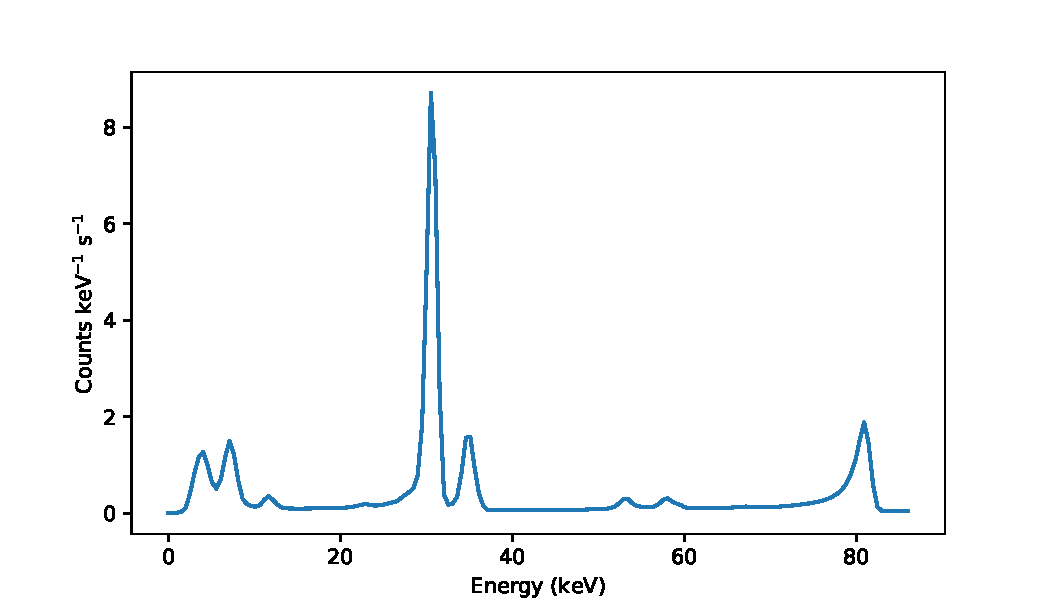
\includegraphics[width=0.8\linewidth]{figures/calibrationSpectrum.pdf}
    \caption{Spectrogram of STIX calibration spectra}
    \label{fig:calibrationSpectrogram}
\end{figure}

calibration data products
https://fermi.gsfc.nasa.gov/ssc/data/access/gbm/
\subsubsection{Solar Orbiter orbit viewer}


When a new data file from the platform is received at the PPDC,
it triggers an autonomous start of the dedicated program that decodes and
interprets its contents. The binary data contain the spacecraft location, attitude, speed, and GPS timestamps with increments every half second. The GPS timestamps are converted into Unix-timestamps, where the leap seconds are also considered. After processing, the platform data are written to the ROOT format files. The data start and stop time, data processing time, input filename and ID of the output file of each processing are recorded in a dedicated database table.
SPICE kernel

Updated once per day.

At the center of the Sun.
It is worth mentioning that has to corrected for.
This can be done by using the web tool provided at the auxiliary data center at


\section{Data access and APIs}
\section{Future work}
\section{Conclusions}




% WARNING
%-------------------------------------------------------------------
% Please note that we have included the references to the file aa.dem in
% order to compile it, but we ask you to:
%
% - use BibTeX with the regular commands:
%   \bibliographystyle{aa} % style aa.bst
%   \bibliography{Yourfile} % your references Yourfile.bib
%
% - join the .bib files when you upload your source files
%-------------------------------------------------------------------

\bibliographystyle{aa}
\bibliography{citations}

\end{document}
